
As shown in homework D.5, the feedback linearized model for the mass-spring-damper is given by 
\begin{equation}\label{eq:soln_d6_1}
m\ddot{z} = \tilde{F} - b\dot{z}
\end{equation}
Taking the Laplace transform of Equation~\eqref{eq:soln_d6_1} and setting all initial conditions to zero we get
\[
ms^2Z(s) = \tilde{F}(s) - bsZ(s).
\]
Solving for $Z(s)$ and putting the transfer function in monic form gives
\begin{equation}\label{eq:soln_d6_2}
Z(s) = \left(\frac{\frac{1}{m}}{s^2 + \frac{b}{m}s}\right)\tilde{F}(s).
\end{equation}
where the expression in the parenthesis is the transfer function from $\tilde{F}$ to $z$, where $\tilde{F}$ indicate that we are working with feedback linearized control derived in homework D.5. The block diagram associated with Equation~\eqref{eq:soln_d6_2} is shown in Figure~\ref{fig:hw_mass_block_diagram}
\begin{figure}[htbp]
   \centering
   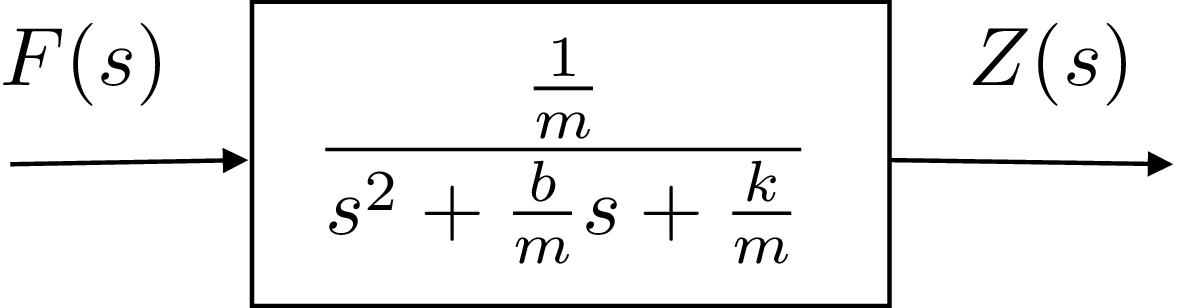
\includegraphics[width=0.4\textwidth]{6_design_studies/figures/hw_mass_block_diagram.pdf}
   \caption{A block diagram of the mass spring damper system.}
   \label{fig:hw_mass_block_diagram}
\end{figure} 
